\chapter{Shortest Paths}%
\label{chap:06}

\section{Examples}
Shortest path algorithms are used in different areas in computer vision, in the
following we briefly discuss two examples. The first example is seeded
segmentation. Consider the Image (a) of the following Figure.

\begin{figure}[H]
  \centering \includegraphics[width=0.9\textwidth]{Figures/cats}
\end{figure}

A user draws the blue and green line to annotate foreground and background,
respectively. Image (b) then shows a for each pixel the similarity to the
foreground class; white means the probability that the particular pixel belongs
to the blue class is high while black means the probability is low (in essence,
this can be seen as a very simple classifier). Based on this image a graph
connecting the pixels in a grid is generated and for each pixel the shortest
path to the closest blue pixel and the closest green pixel is computed. The
total costs of these shortest paths, \ie the distances to the closest blue and
green points are given in the last two images. Blue here means low distance,
green means intermediate distance and red means high distance. Based on these
two images a segmentation into foreground and background can be obtained which
is indicated in the first image as the border around the cat.

Another example is computing a depth map from a stereo image which is discussed
in more detail in Section~\ref{sec:scanline}. The fundamental approach to tackle
shortest path problems is \textbf{dynamic programming}. Generally problems where
dynamic programming techniques are applied are required to have the
\emph{optimal subproblem} property, which means that the optimal solution to a
partial problem has to be part of the overall optimal solution. Consider the
graph in Figure~\ref{fig:shortest_path}. We do not know if the shortest path
from $s$ to $t$ will go through $k$; if it does go through $k$, however, then
the shortest path $s \rightarrow k$ must be part of the globally optimal
shortest path $s \rightarrow t$.
\begin{figure}[htpb]
  \centering
  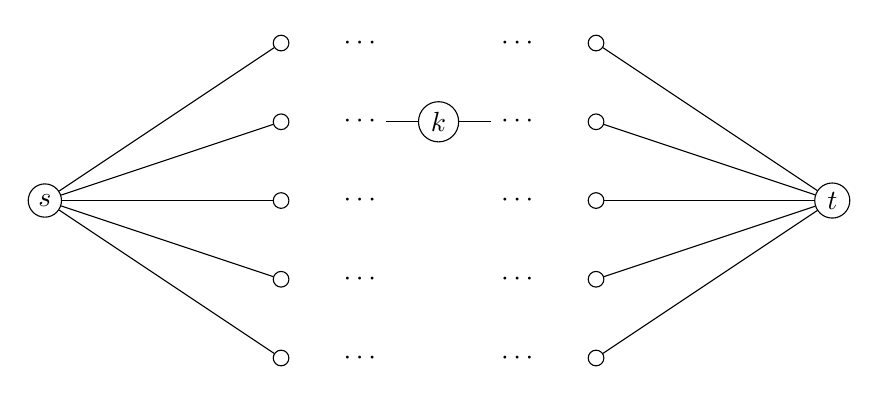
\begin{tikzpicture}
    \node[shape=circle,draw,inner sep=2pt] (S) at (0,0) {$s$};%
    \node[shape=circle,draw,inner sep=2pt] (K1) at (3,2) {};%
    \node[shape=circle,draw,inner sep=2pt] (K2) at (3,1) {};%
    \node[shape=circle,draw,inner sep=2pt] (K3) at (3,0) {};%
    \node[shape=circle,draw,inner sep=2pt] (K4) at (3,-1) {};%
    \node[shape=circle,draw,inner sep=2pt] (K5) at (3,-2) {};%
    \node[shape=circle,draw,inner sep=2pt] (L1) at (7,2) {};%
    \node[shape=circle,draw,inner sep=2pt] (L2) at (7,1) {};%
    \node[shape=circle,draw,inner sep=2pt] (L3) at (7,0) {};%
    \node[shape=circle,draw,inner sep=2pt] (L4) at (7,-1) {};%
    \node[shape=circle,draw,inner sep=2pt] (L5) at (7,-2) {};%
    \node[shape=circle,draw,inner sep=2pt] (K) at (5,1) {$k$};%
    \node[] (C1) at (4,2) {$\cdots$};%
    \node[] (C2) at (4,1) {$\cdots$};%
    \node[] (C3) at (4,0) {$\cdots$};%
    \node[] (C4) at (4,-1) {$\cdots$};%
    \node[] (C5) at (4,-2) {$\cdots$};%
    \node[] (CR1) at (6,2) {$\cdots$};%
    \node[] (CR2) at (6,1) {$\cdots$};%
    \node[] (CR3) at (6,0) {$\cdots$};%
    \node[] (CR4) at (6,-1) {$\cdots$};%
    \node[] (CR5) at (6,-2) {$\cdots$};%
    \node[shape=circle,draw,inner sep=2pt] (T) at (10,0) {$t$};%

    \draw[-] (C2) to (K) to (CR2);%
    \draw[-] (S) to (K1);%
    \draw[-] (S) to (K2);%
    \draw[-] (S) to (K3);%
    \draw[-] (S) to (K4);%
    \draw[-] (S) to (K5);%
    \draw[-] (L1) to (T);%
    \draw[-] (L2) to (T);%
    \draw[-] (L3) to (T);%
    \draw[-] (L4) to (T);%
    \draw[-] (L5) to (T);%
  \end{tikzpicture}
  \caption{We try to find the shortest path from $s$ to $t$. We do not whether
    or not the shortest path will go through $k$ but if it does, }%
  \label{fig:shortest_path}
\end{figure}

Note, that it really only makes sense to use dynamic programming if the
solutions of the subproblems can be re-used multiple times. In methods where the
paths are acyclic, the complexity dynamic programming approach grows only
linearly with the problem size which is the best possible complexity one can
expect.

\section{Shortest Path Algorithms}%
\label{sec:shortpathalgo}
Below we introduce two dynamic programming algorithms that can be used to solve
the shortest path problem. We begin with Viterbi's algorithm which can be
defined in different ways; the version we give below is sometimes referred to as
the forward update version of Viterbi's algorithm.

\begin{algorithm}
  \SetAlgoLined%
  \KwResult{Shortest path starting from node $s$}%
  topologically sort the vertices of $G$\;%
  \ForEach{vertex $v$ in topological order}{%
    \ForEach{edge $e=(u,v)$ in the forward star of $v$}{%
      $d(u) = \min(d(u), d(v) + w(e))$\;%
    }%
  }
  \caption{Viterbi's algorithm}
\end{algorithm}
We start from the node $s$ and follow all edges in the forward star of this
vertex, \ie all outgoing edges. All of these edges connect $s$ to some node $u$
and we now compute the distance from $s$ to $u$ which is given by the edge
weight and possibly and additional weight imposed by the vertex itself. If have
done this for every edge in the forward star of the start node, we now know the
cost for reaching each of its outgoing neighbours. We repeat the process for
each of these vertices, call them $v$, \ie we again follow the edges in the
forward star and compute the distance from $v$ to all nodes $u$ that we can
reach.  Now there are two possibilities. If we have not yet visited the node $u$
through some other path, we simply set the distance of reaching $u$ to the
distance of reaching $v$ plus the edge weight of the edge connecting $v$ and $u$
(and possibly also plus the additional weight of $u$ itself). If, however, we
have already reached $u$ by some other path, we again compute the distance as
above but also compare it with the distance from the other path and only keep
the smaller of both. If we additionally remember for each vertex where we came
from, we can then easily construct the shortest path from any vertex back to the
starting vertex $s$ by simply following this path backwards.

In a later lecture we will discuss this shortest path problem in a more general
setting where the notion of distance and the notion of shortness might be
defined differently. In this case, the algorithm still applies; however, we have
to replace the step where we update the distance by
\begin{equation*}
  d(u) = d(u) \oplus \left( d(v) \otimes w(e) \right)\,,
\end{equation*}
where $\oplus$ and $\otimes$ are generalised operations of what in our case is
the minimum and the sum operation.

In turns out that Viterbi's algorithm can only be used for directed acyclic
graphs, \ie graphs that do not contain any cycles. If the graph does contain
cycles, a similar algorithm called Dijkstra's algorithm can be used. Note that
then the graph must not contain any negative edges since this might lead to
negative cycles which in turn make the notion of shortest path meaningless (the
shortest path would be given by following the negative cycle infinitely many
times).
\todo{Add Pseudocode for Dijkstra}

\section{Scanline Optimisation/ Stereo Disparity Estimation}%
\label{sec:scanline}
We consider the follow situation. There are two cameras, slightly shifted or
rotated and rectified, and they take both take a pictures of the same scene. The
goal is to estimate the ``depth'' of the elements in the scene. As illustrated
in the image in Figure~\ref{fig:stereo_image} below, the two pictures are
evaluated along a horizontal scanline (the example is taken from
\url{http://lunokhod.org/?p=1356}).

\begin{figure}[htpb]
  \centering
  \includegraphics[width=0.9\textwidth]{Figures/input_imagery_and_scanline}
  \caption{Original rectified stereo images.}%
  \label{fig:stereo_image}
\end{figure}

For each pixel along that line, each possible disparity result is evaluated. The
cost of each pixel along a scanline can then be stacked into a matrix; the cost
for each pixel on the scanline in the example image versus each possible
disparity value is shown in Figure~\ref{fig:scanline} below.

\begin{figure}[htpb]
  \centering \includegraphics[width=0.9\textwidth]{Figures/scanline_costs}
  \caption{All possible disparities along one scanline.}%
  \label{fig:scanline}
\end{figure}

The solution for the disparity along this scanline is then the path through this
matrix (image) that has minimum costs (dark areas) with some smoothness
constraint imposed (\ie, the shortest path). The process is repeated for every
horizontal scanline; the resulting disparity map is given in
Figure~\ref{fig:disperity_map}. Since each scanline is treated individually, the
result might be not very smooth in the y-direction and one can apply different
smoothing techniques to obtain a disparity map this is smooth in both the x- and
y-direction.

\begin{figure}[htpb]
  \centering
  \includegraphics[width=0.7\textwidth]{Figures/cones_scanline_optimization_only}%
  \caption{Disparity map for the example above.}%
  \label{fig:disperity_map}
\end{figure}

\section*{MAP -- Maximum a posteriori Estimation}
The problem above can be rewritten as: Find
\begin{align*}
  \min_{z_1, \dotsc, z_n}e(z) &= \min_{z_1, \dotsc, z_n} \sum_{i=1}^{n-1} \psi_{i,i+1}(z_i, z_{i+1}) \\
                              &= \min_{z_1, \dotsc, z_n} \psi_{n-1,n}(z_{n-1}, z_n) + \dotsm + \psi_{2,3}(z_{2}, z_3) + \psi_{0,1}(z_{0}, z_1) \\
                              &= \min_{z_n}\Bigg(
                                \min_{z_{n-1}}\psi_{n-1,n}(z_{n-1},z_n) + \dotsm + \min_{z_2}\Big(
                                \psi_{2,3}(z_2, z_3) + \underbrace{\min_{z_1}\psi_{1,2}(z_1, z_2)}_{
                                m_{1\rightarrow 2}(z_2)
                                }
                                \Big) \dotsm
                                \Bigg)\,,
\end{align*}
where the vectors $z_i$ denote the ``state'' at time $i$ (\ie, the $i$th column
of the graph). Note that the components of these vectors are either one or zero,
and they have to sum up to one. In other words, these state vectors denote in
the end which of the respective nodes of the graph lie in the shortest path (see
also the Figure below).

\begin{figure}[htpb]
  \centering \includegraphics[width=0.6\textwidth]{Figures/state_vectors}
  \caption{State vectors}
\end{figure}

\section{Segmented Least Squares}

%%% Local Variables:
%%% mode: latex
%%% TeX-master: "../main"
%%% End:
